\usetikzlibrary{calc}
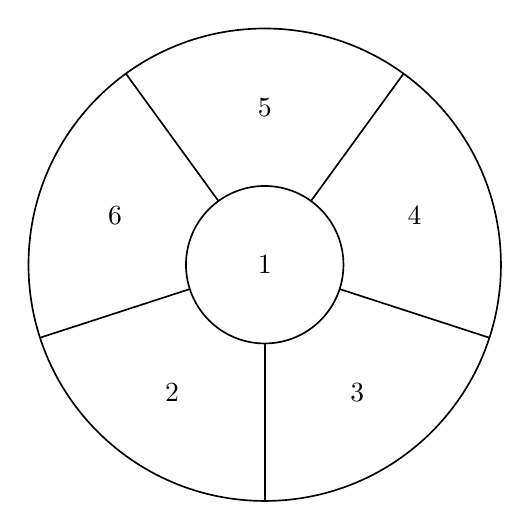
\begin{tikzpicture}[x=1cm,y=1cm,line width=.6pt,font=\normalsize]
\coordinate (O) at (0,0);
\draw (O) circle[radius=3];
\draw (O) circle[radius=1];
\draw (0.5878,0.809) -- (1.7634,2.4271);
\draw (-0.5878,0.809) -- (-1.7634,2.4271);
\draw (-0.9511,-0.309) -- (-2.8532,-0.9271);
\draw (0,-1) -- (0,-3);
\draw (0.9511,-0.309) -- (2.8532,-0.9271);
\node[inner sep=0pt,anchor=center] at (0,0) {$1$};
\node[inner sep=0pt,anchor=center] at (0,2) {$5$};
\node[inner sep=0pt,anchor=center] at (1.9021,0.618) {$4$};
\node[inner sep=0pt,anchor=center] at (1.1756,-1.618) {$3$};
\node[inner sep=0pt,anchor=center] at (-1.1756,-1.618) {$2$};
\node[inner sep=0pt,anchor=center] at (-1.9021,0.618) {$6$};
\end{tikzpicture}
